\setlength{\parindent}{0in}	% disable indentation

\chapter{Traffic danger web system deployment}
\label{cha:systemDeployment}

\section{Environment setup}
\label{sec:environmentSetup}

Java applications are typically compiled to bytecode that can run on any Java Virtual Machine (JVM) regardless of computer architecture. Because of Java platform independence, the system can be deployed on various environments.

\bigskip

For the project to be deployed, following applications should be pre-installed:
\begin{itemize}
    \setlength{\itemsep}{0cm}
    \setlength{\parskip}{0cm}

    \item PostgreSQL database engine,
    \item Java Runtime Environment (JRE),
    \item Apache Tomcat servlet container.
\end{itemize}

\subsection{PostgreSQL installation}
\label{sub:postgreSQLInstallation}

{\scshape Windows}
\smallskip

Get the latest version of PostgreSQL executable package from \url{http://www.postgresql.org/download/windows/}. After downloading simply double click on that package. The installer will do the job.

\bigskip

{\scshape Linux}
\smallskip

Get the latest version of PostgreSQL sources. For the date of writing that file latest version of PostgreSQL was v9.0beta2. Sources can be obtained by anonymous FTP from \url{ftp://ftp.postgresql.org/pub/source/v9.0beta2/postgresql-9.0beta2.tar.gz}. After downloading, unpack the file:
\begin{verbatim}
gzip -dc postgresql-9.0beta2.tar.gz | tar xf -
\end{verbatim}

This will create a directory \texttt{postgresql-9.0beta2} under the current directory with the PostgreSQL sources. Enter into that directory and execute installation procedure:

\newpage

\begin{verbatim}
./configure
gmake
su
gmake install
adduser postgres
mkdir /usr/local/pgsql/data/
chown postgres /usr/local/pgsql/data/
su - postgres
/usr/local/pgsql/bin/initdb -D /usr/local/pgsql/data/
/usr/local/pgsql/bin/postgres -D /usr/local/pgsql/data/ >logfile 2>&1 &
/usr/local/pgsql/bin/createdb test
/usr/local/pgsql/bin/psql test
\end{verbatim}

\subsection{Java Runtime Environment (JRE) installation}
\label{sub:jreInstallation}

Download the Java 2 Standard Edition Runtime (JRE) release version 5.0 or later, from \url{http://www.java.com/en/download/manual.jsp} and install the JRE according to the instructions included with the release. 

\bigskip

Set the environment variable named \texttt{JRE\_HOME} to the pathname of the directory into which you installed the JRE, e.g.

\bigskip

{\scshape Linux}
\begin{verbatim}
# for Bourne, bash, and related shells
export JRE_HOME=/usr/local/java/jre5.0
\end{verbatim}
\begin{verbatim}
# for csh and related shells
setenv JRE_HOME=/usr/local/java/jre5.0
\end{verbatim}

{\scshape Windows}
\begin{verbatim}
set JRE_HOME=C:\jre5.0
\end{verbatim}

You can also use the full JDK rather than just the JRE. In this case set the \texttt{JAVA\_HOME} environment variable to the pathname of the directory into which you installed the JDK.

\subsection{Apache Tomcat installation}
\label{sub:apacheTomcatInstallation}

Download the latest version of Tomcat binary distribution from \url{http://tomcat.apache.org/}, appropriate for your system and unpack the file into convenient location so that the distribution resides in its own directory:

\bigskip

{\scshape Linux}
\begin{verbatim}
cp apache-tomcat-6.0.26.tar.gz /usr/local/apache/
cd /usr/local/apache/
gzip -dc apache-tomcat-6.0.26.tar.gz | tar xf -
\end{verbatim}

\bigskip

Set the \texttt{CATALINA\_HOME} environmental variable (it is used to refer to the full pathname of the release directory):

\bigskip

{\scshape Linux}
\begin{verbatim}
# for Bourne, bash, and related shells
export CATALINA_HOME=/usr/local/apache/apache-tomcat-6.0.26
\end{verbatim}
\begin{verbatim}
# for csh and related shells
setenv CATALINA_HOME=/usr/local/apache/apache-tomcat-6.0.26
\end{verbatim}

{\scshape Windows}
\begin{verbatim}
set CATALINA_HOME=C:\apache\apache-tomcat-6.0.26
\end{verbatim}

\bigskip

{\large\textbf{Startup Tomcat:}}

\bigskip

{\scshape Linux}
\begin{verbatim}
$CATALINA_HOME/bin/startup.sh
\end{verbatim}

{\scshape Windows}
\begin{verbatim}
%CATALINA_HOME%\bin\startup.bat
\end{verbatim}

After starting the default web applications included with Tomcat will be available at address: \url{http://localhost:8080/}

\bigskip

\begin{framed}
If Tomcat is not responding, the reason can be another web server (or process) running and using provided port \texttt{8080}. The solution is to edit \path{$CATALINA_HOME/conf/server.xml} configuration file and change the default port.
\end{framed}

\bigskip

{\large\textbf{Shutdown Tomcat:}}

\bigskip

{\scshape Linux}
\begin{verbatim}
$CATALINA_HOME/bin/shutdown.sh
\end{verbatim}

{\scshape Windows}
\begin{verbatim}
%CATALINA_HOME%\bin\shutdown.bat
\end{verbatim}

\newpage

\section{Loading and configuration}
\label{sec:loadingAndConfiguration}

Open the \textit{Tomcat Manager} available under the \textit{Tomcat Administration} panel at address \url{http://localhost:8080/manager/html/}:

\begin{framed}
If you are not authorized to view this page, you should probably examine \path{$CATALINA_HOME/conf/tomcat_users.xml} file and, if necessary, define a new user with appropriate rights, e.g. \texttt{<user username="root" password="toor" roles="manager-gui" />}.
\end{framed}

\begin{figure}[htp]
\centering
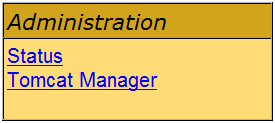
\includegraphics[scale=0.6]{images/appendixA/TomcatAdministration}
\caption{Tomcat administration panel}
\label{fig:tomcatAdministrationPanel}
\end{figure}

Under the \textit{WAR file to deploy} section shown in Figure \ref{fig:WARArchiveDeployment}, deploy \texttt{traffic\_web-1.0.0.war} archive, containing prebuild web application for traffic danger web system.

\medskip

\begin{figure}[htp]
\centering
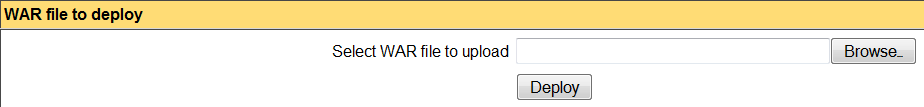
\includegraphics[scale=0.5]{images/appendixA/WARArchiveDeployment}
\caption{WAR archive deployment section}
\label{fig:WARArchiveDeployment}
\end{figure}

\bigskip

After deployment is complete, open for edition \path{$CATALINA_HOME/webapps/traffic_web/WEB-INF/web.xml} file and change value of \texttt{OntologyURI} parameter for appropriate path indicating ontology file for traffic danger \texttt{TrafficDanger.owl}. 

\bigskip

The URI can identify local or remote resource, for example:
\begin{itemize}
    \setlength{\itemsep}{0cm}
    \setlength{\parskip}{0cm}

    \item \path{file:///C:/Users/jwa/masters/TrafficDanger.owl} (local Windows location),
    \item \path{file:///home/jwa/masters/TrafficDanger.owl} (local Linux location),
    \item \path{http://host/TrafficDanger.owl} (remote location).
\end{itemize}

\smallskip

Final step is about SQL scripts execution, required for database creation. Run the following scripts in the given order: \texttt{postgres\_traffic\_user.sql}, \texttt{postgres\_traffic\_database.sql}, \texttt{postgres\_traffic\_schema.sql} and finally \texttt{postgres\_traffic\_data.sql}. The last one actually contains sample data, so its execution is optional.

\newpage

{\scshape Linux}
\smallskip

Change user to \texttt{postgres}, and change catalog to directory containing database scripts and invoke following commands:

\begin{verbatim}
psql -f postgres_traffic_user.sql
psql -f postgres_traffic_database.sql
psql -f postgres_traffic_schema.sql traffic
psql -f postgres_traffic_data.sql traffic
\end{verbatim}

After that, system should be ready to cooperate under address \url{http://localhost:8080/traffic_web-1.0.0/board.html}.
